\documentclass{beamer}
\usepackage[orientation=portrait,size=a0,debug]{beamerposter}
\mode<presentation>{\usetheme{ZH}}

\usepackage[utf8]{inputenc}
\usepackage[english, russian]{babel} % required for rendering German special characters
\usepackage[T2A]{fontenc}
\usepackage{subcaption}
\usepackage{wrapfig}
\usepackage{url}

\usepackage{siunitx} %pretty measurement unit rendering
\usepackage{hyperref} %enable hyperlink for urls
\usepackage{ragged2e}
\usepackage[font=scriptsize,justification=justified]{caption}
\usepackage{array, booktabs, tabularx}

\newcolumntype{Z}{>{\centering\arraybackslash}X} % centered tabularx columns
\sisetup{per=frac,fraction=sfrac}

\title{\huge Анализ активности аккрецирующих рентгеновских пульсаров и черных дыр}
\author{Киселев Владимир \hfill Научный руководитель: к. ф.-м. Свинкин Дмитрий Сергеевич}
\institute[PTHS]{$^{1}$ Академический лицей <<Физико-техническая школа>>}
\date{10.03.2019}

% edit this depending on how tall your header is. We should make this scaling automatic :-/
\newlength{\columnheight}
\setlength{\columnheight}{104cm}

\begin{document}
\begin{frame}
\begin{columns}
	\begin{column}{.43\textwidth}
		\begin{beamercolorbox}[center]{postercolumn}
			\begin{minipage}{.98\textwidth}  % tweaks the width, makes a new \textwidth
				\parbox[t][\columnheight]{\textwidth}{ % must be some better way to set the the height, width and textwidth simultaneously
					\begin{myblock}{Введение}
						Аккрецирующие рентгеновские пульсары --- быстро вращающиеся нейтронные звезды с сильным магнитным полем ($\sim10^{12} - 10^{13}$ Гс), у которых есть так называемый аккреционный диск.
						
						Аккреционный диск является газом, перетекающим со звезды-компаньона на компактный объект (белый карлик, нейтронная звезда, черная дыра).	
						
						\begin{figure}
							\centering
							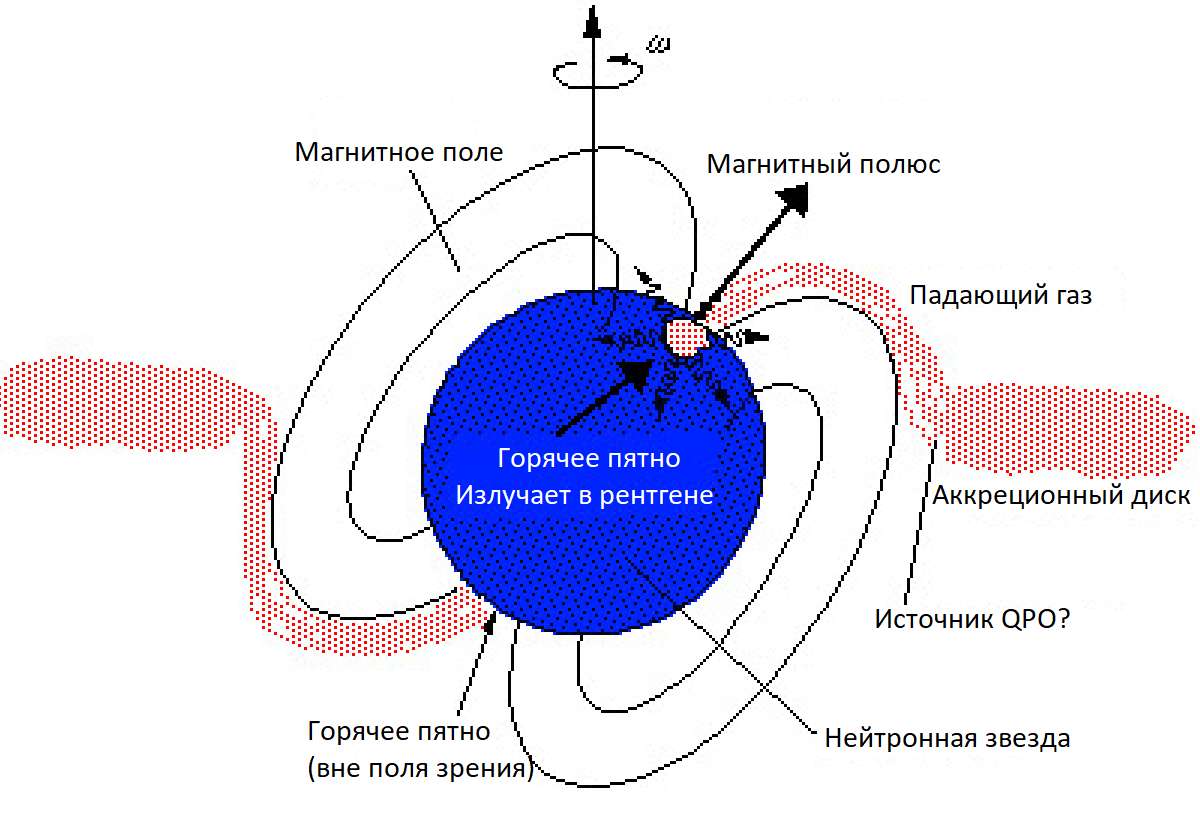
\includegraphics[width=0.8\textwidth]{img/accretion_pulsar}			
							\caption{Аккрецирующий рентгеновский пульсар и его составляющие}
						\end{figure}
						
						\vspace{0.4em}
						
						Одним из представителей тесной двойной системы (компактный объект и звезда-компаньон) является кандидат в черную дыру MAXI J1820+070.
						
						MAXI J1820+070 был впервые зарегистрирован 11 марта 2018 года с помощью прибора MAXI. Вспышка такого объекта была видна в различных диапазонах волн и различными обсерваториями. К примеру, на рис. \ref{img:bh} представлена вспышка, которую зафиксировал прибор MAXI/GSC.
						
						\begin{figure}[h!]
							\centering
							\begin{subfigure}[b]{0.4\linewidth}
								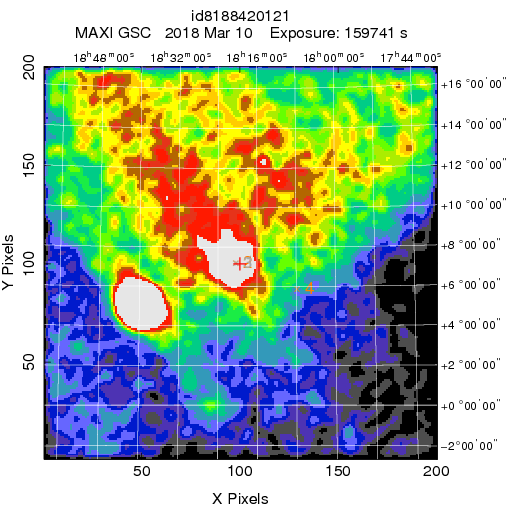
\includegraphics[width = \textwidth]{pictures/maxij_image_full.png}
								\caption{}
								\label{img:bhfull}
							\end{subfigure}
							\begin{subfigure}[b]{0.4\linewidth}
								\centering
								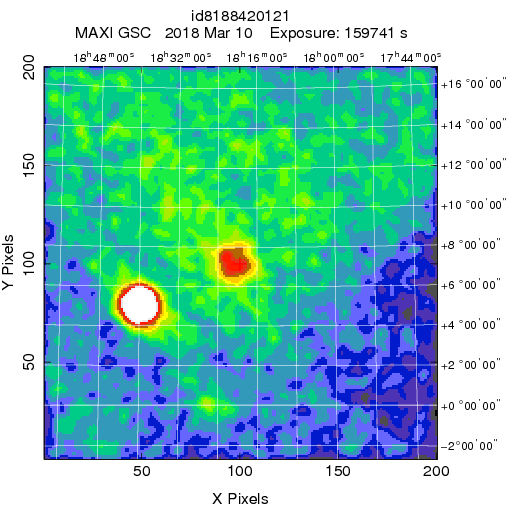
\includegraphics[width = \textwidth]{pictures/maxij_image.png}
								\caption{}
							\label{img:bhpart}
							\end{subfigure}
							\caption{Область неба, в которой был обнаружен MAXI J1820+070 в диапазоне от 2 до 20 кэВ (а) и диапазоне от 2 до 4 кэВ (b)}
							\label{img:bh}
						\end{figure}
						
						В ходе наблюдений за объектом было замечено, что  MAXI J1820+070 является источником QPO. QPO или, по-другому, квазипериодические колебания были в открыты в начале 80-х годах у нескольких маломассивных рентгеновских двойных. В отличие от периодического излучения, излучение этих объектов меняется в каких-то пределах, т.е. можно назвать это <<квазиколебаниями>> с <<квазипериодом>> обычно от $\thicksim 0.1$ до $\thicksim 0.01$ Гц. Изначально QPO были найдены у нейтронных звезд, но при дальнейшем изучении также и у кандидатов в черные дыры.
					\end{myblock}\vfill
					\begin{myblock}{Методика}
						
						Суть работы заключается в анализе данных наблюдений рентгеновских пульсаров и кандидатов в черные дыры с космических аппаратов, дальнейшее определение параметров таких особенностей компактных объектов, как квазипериодические осцилляции и их эволюция со временем.
						
						Данные представляют собой несколько массивов чисел, означающих количество считанных фотонов за единицу времени на разных энергетических диапазонах.
	
						Для анализа квазипериодических осцилляций используется спектр мощности сигнала, полученный из временных историй скоростей счёта гамма-квантов преобразованием Фурье (или по-другому FFT).
						\begin{figure}
							\centering
							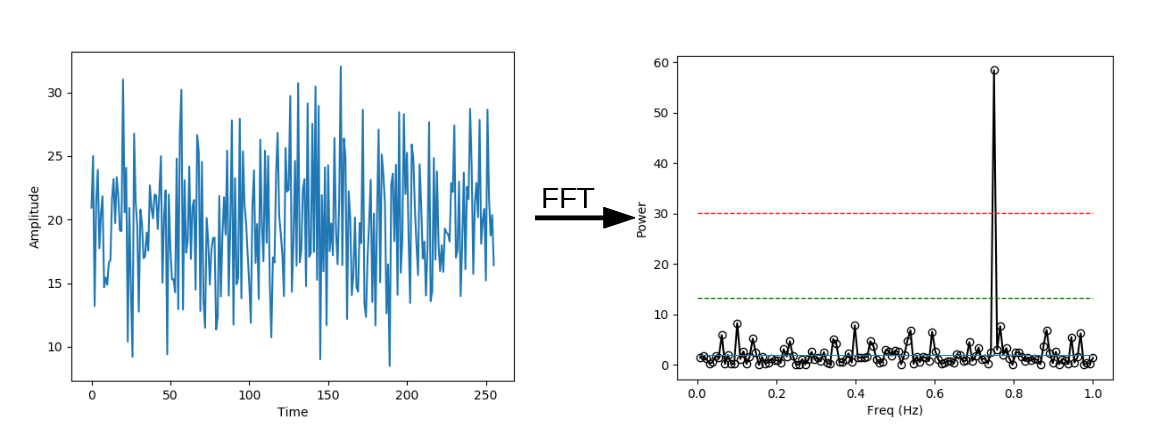
\includegraphics[width=0.85\textwidth]{FFT}
							\caption{Преобразование Фурье помогает понять является ли сигнал периодическим и если да, то с какой частотой излучает объект}
						\end{figure}
	
						При анализе кандидата в черную дыру временная история разбивается на равные части определенной длительности (в нашем случае --- 1 день). Для каждого участка строится его спектр мощности, который затем аппроксимируется степенной функцией вида $f^{-1}$ и распределением Гаусса при помощи так называемого метода наибольшего правдоподобия. В результате выполнения программы находится частота квазипериодических колебаний.
						
						\begin{figure}
							\centering
							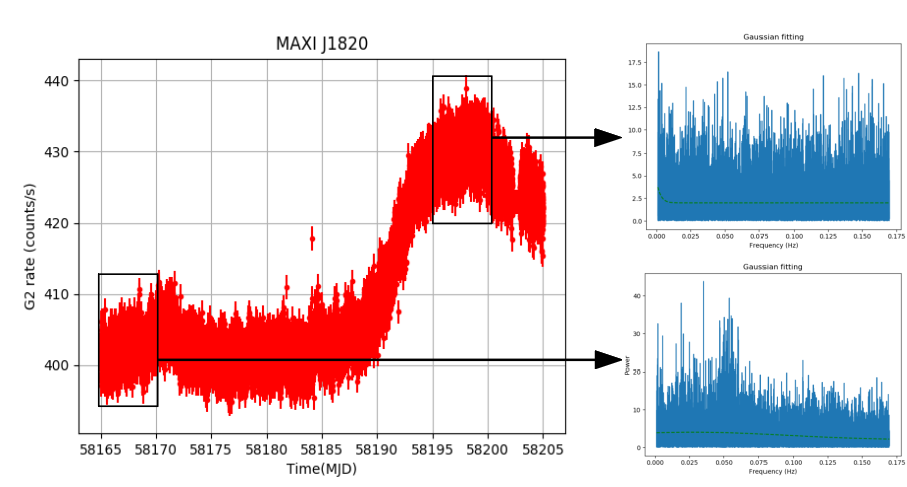
\includegraphics[width=0.9\textwidth]{example.png}
							\caption{Красным обозначены данные с прибора, а синим график зависимости мощности от частоты после преобразования Фурье выделенной черным прямоугольником области}
							\label{fig:graf}
						\end{figure}

						
					\end{myblock}\vfill
		}\end{minipage}\end{beamercolorbox}
	\end{column}
	\begin{column}{.57\textwidth}
		\begin{beamercolorbox}[center]{postercolumn}
			\begin{minipage}{.98\textwidth} % tweaks the width, makes a new \textwidth
				\parbox[t][\columnheight]{\textwidth}{ % must be some better way to set the the height, width and textwidth simultaneously
					\begin{myblock}{Инструменты}
						
						Конус --- гамма-спектрометр, установленный на космический аппарат \textit{GGS-Wind}. Данные с этого прибора можно увидеть на рис. \ref{fig:graf}.
						
						BAT --- один из инструментов орбитальной обсерватории SWIFT, представляющий из себя телескоп с кодирующей маской. Данный прибор также наблюдал MAXI J1820+070 и изначально данные с Konus-Wind сравнивались с Swift/BAT.
						
						\begin{figure}[h!]
							\centering
							\begin{subfigure}[b]{0.59\linewidth}
								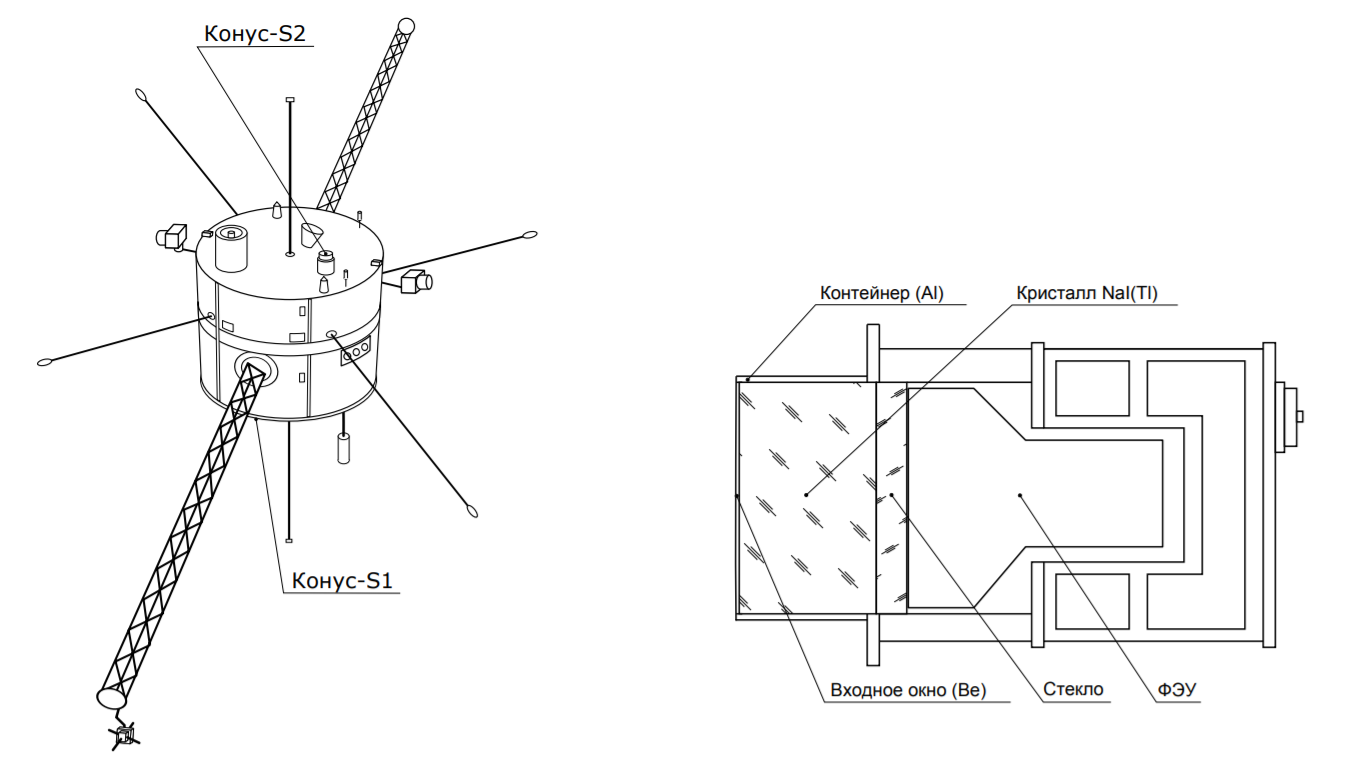
\includegraphics[width = \linewidth]{pictures/Konus-Wind.png}
								\caption{Устройство (слева) спутника \textit{GGS-Wind} и (справа) самого прибора}
							\end{subfigure}
							\begin{subfigure}[b]{0.38\linewidth}
								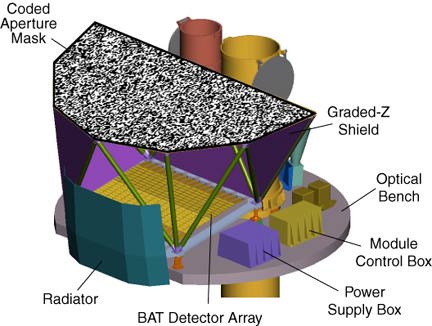
\includegraphics[width = \textwidth]{pictures/BAT.jpg}
								\caption{Устройство прибора BAT}
							\end{subfigure}
						\end{figure}

					\end{myblock}\vfill
					\begin{myblock}{Результаты}
					
						В итоге сделана программа для анализа периодических сигналов, поиска значимых гармоник и их аппроксимация для дальнейшего нахождения пика QPO. Также сравнены данные по MAXI J1820+070, полученные с инструментов Konus-Wind, Swift/BAT, INTEGRAL/ISGRI, что можно увидеть ниже. Интересно то, что, несмотря на одинаковый спектр регистрируемых фотонов у ISGRI и Konus-Wind, первый прибор после пика регистрировал больше фотонов, чем второй.
	
						\begin{figure}[h!]
							\begin{subfigure}[b]{0.45\textwidth}
								\centering
								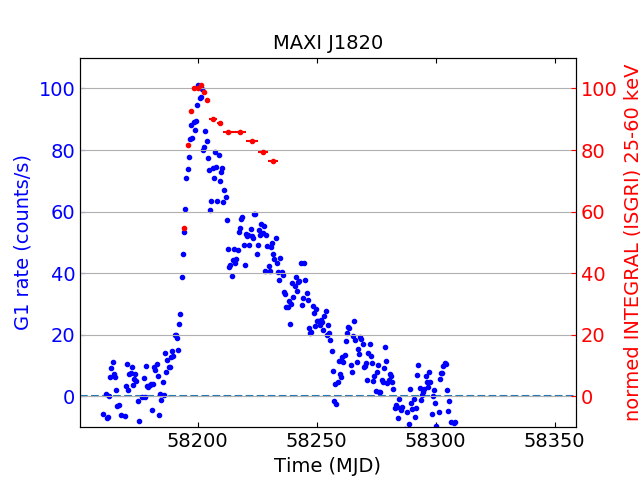
\includegraphics[width=\textwidth]{pictures/MAXIJ1820_kwG1_int.png}
								\caption{}
							\end{subfigure}
							\begin{subfigure}[b]{0.45\textwidth}
								\centering
								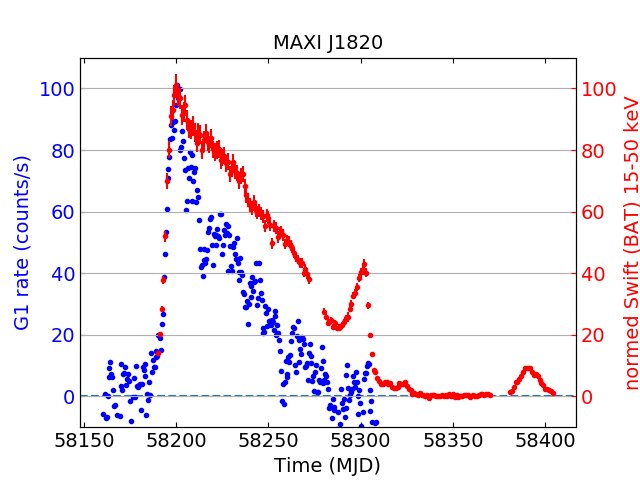
\includegraphics[width=\textwidth]{pictures/MAXIJ1820_kwG1_bat.png}
								\caption{}				
							\end{subfigure}
							\caption{Сравнение счета фотонов у Конус-Винд c (a) INTEGRAL или (b) BAT}
						\end{figure}
						
						Изначально была дана информация о первых 130 днях наблюдения за MAXI J1820+070. После разбиения сигнала на 130 однодневных сигналов, оказалось, что на 38-ой день в спектре мощности можно найти квазипериодические осцилляции. Их возможно обнаружить до 62 дня. Частота осцилляций увеличивалась со временем от $0{,}03$ до $0{,}10$ Гц.
						
						При построении графика зависимости частоты квазипериодических осцилляций от времени, получается, что она возрастает со временем.
						\begin{figure}[h]
							\centering
							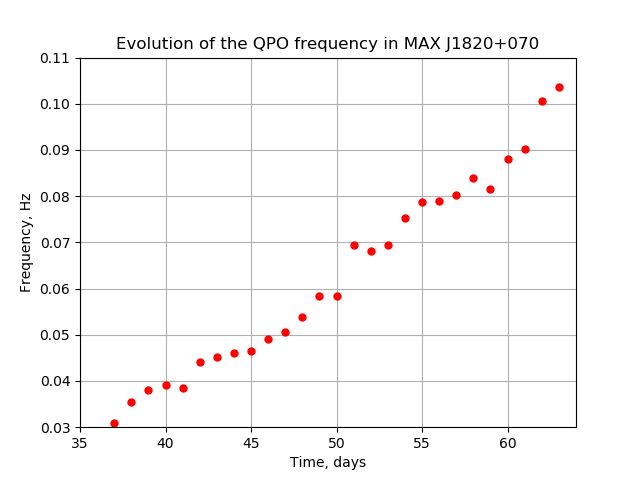
\includegraphics[width=0.4\linewidth]{result}
							\caption{График зависимости частоты квазипериодических колебаний от времени}
						\end{figure}
						
						Скрипт и остальные графики аппроксимации расположены в Github: 
						\url{https://github.com/Grindegreen/report}
					
					\end{myblock}\vfill
					\begin{myblock}{Интерпретация результатов}
						
						Исследование квазипериодических осцилляций позволяет изучать аккреционный поток вокруг черных дыр иным способом, нежели чем энергетический спектр. Соответствие QPO с конкретными спектральными состояниями и переходами между ними может помочь понять физические условия, приводящие к ним, поскольку на данный момент.
						
						Систематические изменения яркости (вспышка, например) в спектре черной дыры являются следствием  изменений в аккреционном диске. Само состояние можно описать с помощью шаблонов отслеживаемых на диаграмме твердости-интенсивности. Под интенсивностью подразумевается скорость счета фотонов, а под твердостью подразумевается эквивалент фотометрического индекса цвета. На рис. \ref{img:sz} показана типичная форма кривой диаграммы.
							\begin{figure}[h!]
								\centering
								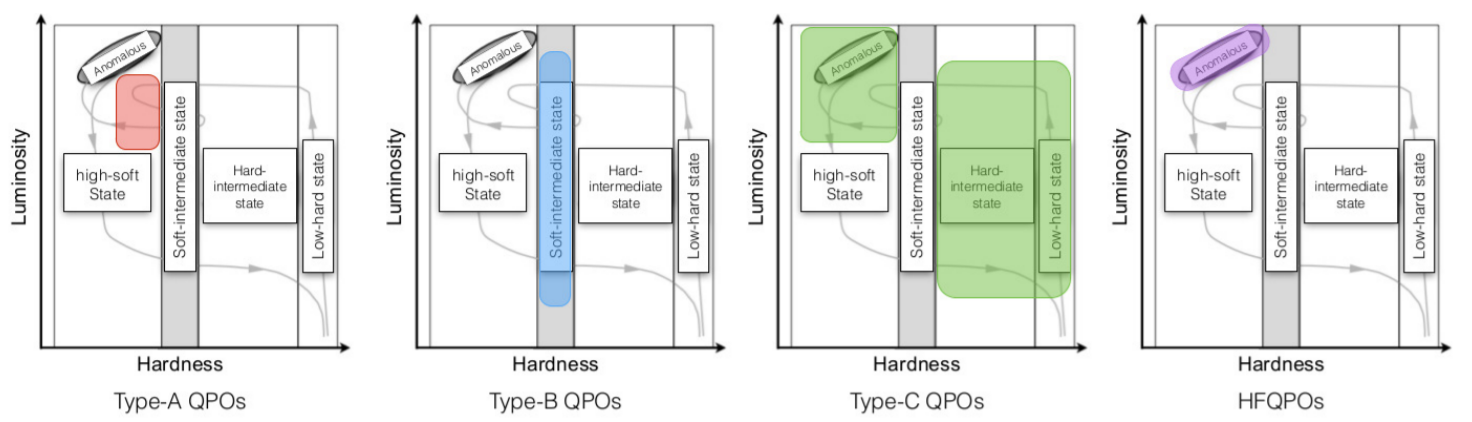
\includegraphics[width = \linewidth]{pictures/HID.png}
								\caption{Типичная диаграмма твердости-интенсивности для черной дыры. Кривая поделена на пять спектральных состояний, также отмечено в каком состоянии проявляются какие QPO}
								\label{img:sz}
							\end{figure}
	
							Пять спектральных состояний, показанных на рисунке различаются по способу излучения, а именно:
	
							\begin{itemize}
								\item 	Low Hard. В этом состоянии основной источник излучения --- комптоновская эмиссия
								\item High Soft. Здесь источник излучения --- нагретый аккреционный диск
								\item Hard Intermediate и Soft Intermediate. В этих двух состояниях спектр состоит как из жесткого компонента (джет, например), так и теплового излучения диска.
								\item Аномальное. Отличие от Hard Intermediate и Soft Intermediate состоит в том, что светимость объекта значительно выше, чем при последних. 
							\end{itemize}
	
							Квазипериодические осцилляции разделяют на несколько типов: A, B, C и высокочастотные осцилляции. Каждый из типов осцилляций характерен для своего спектрального состояния черной дыры.
							
							Для типа C характерны частоты, которые и были обнаружены у MAXI J1820+070, из чего можно сделать вывод, что черная дыра на момент наблюдения находилась в состоянии HIS.
						
					\end{myblock}\vfill
		}\end{minipage}\end{beamercolorbox}
	\end{column}
\end{columns}
\end{frame}
\end{document}